\hypertarget{3.3}{\subsection{Das Taxas de Juros e Correção Aplicadas em cotejo com a Taxa SELIC}}

Conforme constatado no tópico anterior, a \textbf{FESP} aplicou na data da lavratura do AIIM de n° 4.037.656-4 taxas nos patamares de \textbf{14,78\%}, tanto para cálculo dos juros sobre o principal como para a atualização do valor básico para cálculo da multa punitiva, sendo esta a controvérsia que origina o exame pericial no caso em tela, uma vez que se alega na exordial que referida taxa supera os patamares da Taxa SELIC.

Neste diapasão, eximindo-se de quaisquer juízos de valor quanto à aplicabilidade ou não da Taxa SELIC em substituição às taxas adotadas pela \textbf{Requerida}, sendo esta atribuída oportunamente ao Juízo, a \textbf{Perícia} perseguiu na própria fonte de cálculo dos débitos tributários administrados pela União, qual seja o sítio da Receita Federal do Brasil, obtendo o que segue:

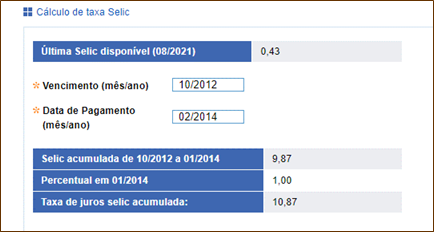
\includegraphics{Imagens/Figura 1 Taxa SELIC acumulada extraída do SICALC (Programa de Atualização Débitos da RFB).png}
%indentar texto abaixo:

\textbf{Constatação:} Constata-se que, considerando o termo inicial em outubro de 2012 (mês de competência das transações autuadas) e o mês da lavratura do AIIM (fevereiro de 2014), a Taxa SELIC Acumulada nos moldes estabelecidos pela União para os juros e correção dos débitos tributários perfaz \textbf{10,87\%} na data da lavratura do AIIM.
%Fim da indentação

Dessa forma, para fins de comparação entre o cálculo original do AIIM \textit{sub judice} (pautado na Lei Estadual nº 13.918/2009) e a tese da \textbf{Requerente} que requer limitação dos juros e correção aos patamares da Taxa SELIC (Arguição de Inconstitucionalidade nº 0170909-61.212.8.26.000), a Perícia substituiu o \textbf{percentual de 14,78\% (originário) por 10,87\% (Taxa SELIC acumulada conforme Receita Federal do Brasil)}, vejamos:

\begin{table}[h!]
    \centering
    \resizebox{\textwidth}{!}{
    \begin{tabular}{|m{1cm}|m{2cm}|m{1.7cm}|m{1cm}|m{1.4cm}|m{1.7cm}|m{2cm}|m{1.cm}|m{1.6cm}|m{1cm}|m{1cm}|m{2cm}|}
        \hline
        Item do AIIM & Valor Original do Tributo (R\$) & Termo Inicial Juros & Taxa Juros SELIC (\%) & Valor dos Juros (R\$) & Valor Básico Multa (R\$) & Termo Inicial – Multa & Taxa (\%) & Valor Básico Atualizado (R\$) & Multa (\%) & Valor Multa (R\$) \\ \hline
        
        1 &	138.240,00 & 31/10/2012 & 10,87 & 15.026,69 & 844.800,00 &  31/10/2012 & 10,87 & 936.629,76 & 50,00 & 468.314,88 \\ \hline
        
        Total & 138.240,00 & & & 15.026,69 & 844.800,00 & & & 936.629,76 & & 468.314,88 \\ \hline
    \end{tabular}}
    \caption{Recálculo do Anexo ao AIIM n° 4.037.656-4 em 26/02/2014}
    \label{tab:my_label}
\end{table}

%Texto a ser indentado
\textbf{Constatação:} Constata-se que, aplicando a taxa de \textbf{10,87\%} identificada no próprio programa que acumula a Taxa SELIC e que remunera os débitos federais (tese da \textbf{Requerente)}, o resultado de juros perfaz o montante de \textbf{R\$ 15.026,69} enquanto o valor básico da multa punitiva atualizado em fevereiro de 2014 resulta no montante de
\textbf{R\$ 936.629,76}, figurando como base de cálculo para aplicabilidade da multa calculada em \textbf{R\$ 468.314,88}.
%fim da indentação

Dessa forma, visando ilustrar a comparação entre os valores resultantes do AIIM originário e aqueles calculados pela \textbf{Perícia} consoante tese da Requerente, vejamos a tabela a seguir:

\hypertarget{tab3}{}
\begin{table}[h!]
    \centering
    %\resizebox{\textwidth}{!}{
    \begin{tabular}{|m{2cm}|m{2cm}|m{1.7cm}|m{1.5cm}|}
        \hline
        Origem & Valor dos Juros (R\$) & Valor da Multa (R\$) & Diferença Total (R\$) \\ \hline
        
        AIIM Original & 20.431,87 & 484.830,72 & \\ \hline
        
        AIIM Recálculo & 15.026,69 & 468.314,88 & \\ \hline
        
        DIFERENÇA & 5.405,18 & 16.515,84 & 21.921,02 \\ \hline
    \end{tabular}
    %}
    \caption{Resumo da comparação entre Juros e Multa do AIIM Original em cotejo com o Recálculo (Taxa SELIC)}
    \label{tab:my_label}
\end{table}

%Texto a ser indentado
\textbf{Constatação:} Constata-se que, entre o cálculo do AIIM originário e o recálculo da \textbf{Perícia}, apura-se uma diferença de juros exigidos a maior da \textbf{Requerente} em \textbf{R\$ 5.405,18}, da mesma forma apurando-se a diferença a maior de \textbf{R\$ 16.515,84} a título de multa punitiva, totalizando uma diferença de \textbf{R\$ 21.921,02} na data-base 26/02/2014 (data da lavratura).
% Fim do texto a ser indentado

Portanto, conclui-se que \emph{o percentual de 14,78\% adotado como taxa juros} aplicada sobre o principal do imposto e adotada para correção do valor básico (base de cálculo) da multa punitiva \emph{é superior aos patamares da Taxa SELIC que, para o mesmo período de lavratura do AIIM, resulta em 10,87\%} consoante parâmetros estabelecidos pela Receita Federal do Brasil (União), nos termos da Arguição de Inconstitucionalidade nº 0170909-61.212.8.26.000, ofertando à V. Exa. o resultado deste e ficando este \textbf{signatário} à disposição para as atualizações que julgar necessárias.